\section{Result}

\subsection{Measurements for spring constant}

First we get the raw length measurement data in Table~\ref{s1}.
\begin{table}[H]
	\centering
	\begin{tabular}{|p{0.7cm}|p{3cm}||p{0.7cm}|p{3cm}||p{0.7cm}|p{3cm}|}
	\hline
	\multicolumn{2}{|c|}{spring 1 [cm] $\pm$ 0.01 [cm]} &
	\multicolumn{2}{|c|}{spring 2 [cm] $\pm$ 0.01 [cm]} &
	\multicolumn{2}{|c|}{serial   [cm] $\pm$ 0.01 [cm]} \\ \hline
	$L_0$ & 0.00  & $L_0$ & 0.00  & $L_0$ & 20.00 \\ \hline
	$L_1$ & 2.00  & $L_1$ & 2.01  & $L_1$ & 23.96 \\ \hline
	$L_2$ & 3.96  & $L_2$ & 4.00  & $L_2$ & 27.94 \\ \hline
	$L_3$ & 5.96  & $L_3$ & 6.03  & $L_3$ & 31.90 \\ \hline
	$L_4$ & 8.02  & $L_4$ & 8.06  & $L_4$ & 36.40 \\ \hline
	$L_5$ & 10.04 & $L_5$ & 10.08 & $L_5$ & 39.94 \\ \hline
	$L_6$ & 12.02 & $L_6$ & 12.10 & $L_6$ & 44.02 \\ \hline
	\end{tabular}
	\caption{Spring constant measurement data}
\label{s1}
\end{table}

Then we can calculate the change amount of the spring length by $\Delta L_i=L_i-L_0$ and get Table \ref{s2}.

\begin{table}[H]
	\centering
	\begin{tabular}{|p{0.7cm}|p{3cm}||p{0.7cm}|p{3cm}||p{0.7cm}|p{3cm}|}
	\hline
	\multicolumn{2}{|c|}{spring 1 [cm] $\pm$ 0.01 [cm]} &
	\multicolumn{2}{|c|}{spring 2 [cm] $\pm$ 0.01 [cm]} &
	\multicolumn{2}{|c|}{serial   [cm] $\pm$ 0.01 [cm]} \\ \hline
	$\Delta L_1$ & 2.00  & $\Delta L_1$ & 2.01  & $\Delta L_1$ & 3.96  \\ \hline
	$\Delta L_2$ & 3.96  & $\Delta L_2$ & 4.00  & $\Delta L_2$ & 7.94  \\ \hline
	$\Delta L_3$ & 5.96  & $\Delta L_3$ & 6.03  & $\Delta L_3$ & 11.90 \\ \hline
	$\Delta L_4$ & 8.02  & $\Delta L_4$ & 8.06  & $\Delta L_4$ & 16.40 \\ \hline
	$\Delta L_5$ & 10.04 & $\Delta L_5$ & 10.08 & $\Delta L_5$ & 19.94 \\ \hline
	$\Delta L_6$ & 12.02 & $\Delta L_6$ & 12.10 & $\Delta L_6$ & 24.02 \\ \hline
	\end{tabular}
	\caption{Calculated Spring constant measurement data}
\label{s2}
\end{table}

We get the mass of the weight object for every $\Delta L_i$ in Table
\ref{massofweight}.

Since the acceleration due to gravity in Shanghai is $9.794 m/s^2$, we calculated
the weights of each weight object from its mass, as shown in Table
\ref{gravityofweight}. 

\begin{minipage}{0.5\linewidth}
	\begin{table}[H]
	\centering
	\begin{tabular}{|c|c|}
	\hline
	\multicolumn{2}{|c|}{m [g] $\pm$ 0.01 [g]} \\ \hline
	1 & 4.65  \\ \hline
	2 & 9.32  \\ \hline
	3 & 14.17 \\ \hline
	4 & 18.99 \\ \hline
	5 & 23.80 \\ \hline
	6 & 28.51 \\ \hline
	\end{tabular}
	\caption{Mass measurement data.}
\label{massofweight}
	\end{table}
\end{minipage}
%
\begin{minipage}{0.5\linewidth}
	\begin{table}[H]
	\centering
	\begin{tabular}{|c|c|}
	\hline
	\multicolumn{2}{|c|}{F [N] $\pm$ 0.0001 [N]} \\ \hline
	1  & 0.0455  \\ \hline 
	2  & 0.0913  \\ \hline 
	3  & 0.1388  \\ \hline 
	4  & 0.1860  \\ \hline 
	5  & 0.2331  \\ \hline 
	6  & 0.2792  \\ \hline 
	\end{tabular}
	\caption{Weight measurement data.}
\label{gravityofweight}
\end{table}
\end{minipage}


% =====================================
% NOTE: Spring 1
For Spring 1, we can have its length change data versus the force affected on it
data.  

\begin{table}[H]
	\centering
	\begin{tabular}{|c|c|c|}
	\hline
	No. & length [cm] $\pm$ 0.01 [cm] & F [N] $\pm$ 0.0001 [N] \\ \hline
	$\Delta L_1$ & 2.00  &  0.0455  \\ \hline
	$\Delta L_2$ & 3.96  &  0.0913  \\ \hline
	$\Delta L_3$ & 5.96  &  0.1388  \\ \hline
	$\Delta L_4$ & 8.02  &  0.1860  \\ \hline
	$\Delta L_5$ & 10.04 &  0.2331  \\ \hline
	$\Delta L_6$ & 12.02 &  0.2792  \\ \hline
	\end{tabular}
	\caption{$\Delta L$  vs. Force for Spring 1}
\label{s1df}
\end{table}

Then we use MATLAB fit tools to find $k_1$

\begin{figure}[H]
	\centering
	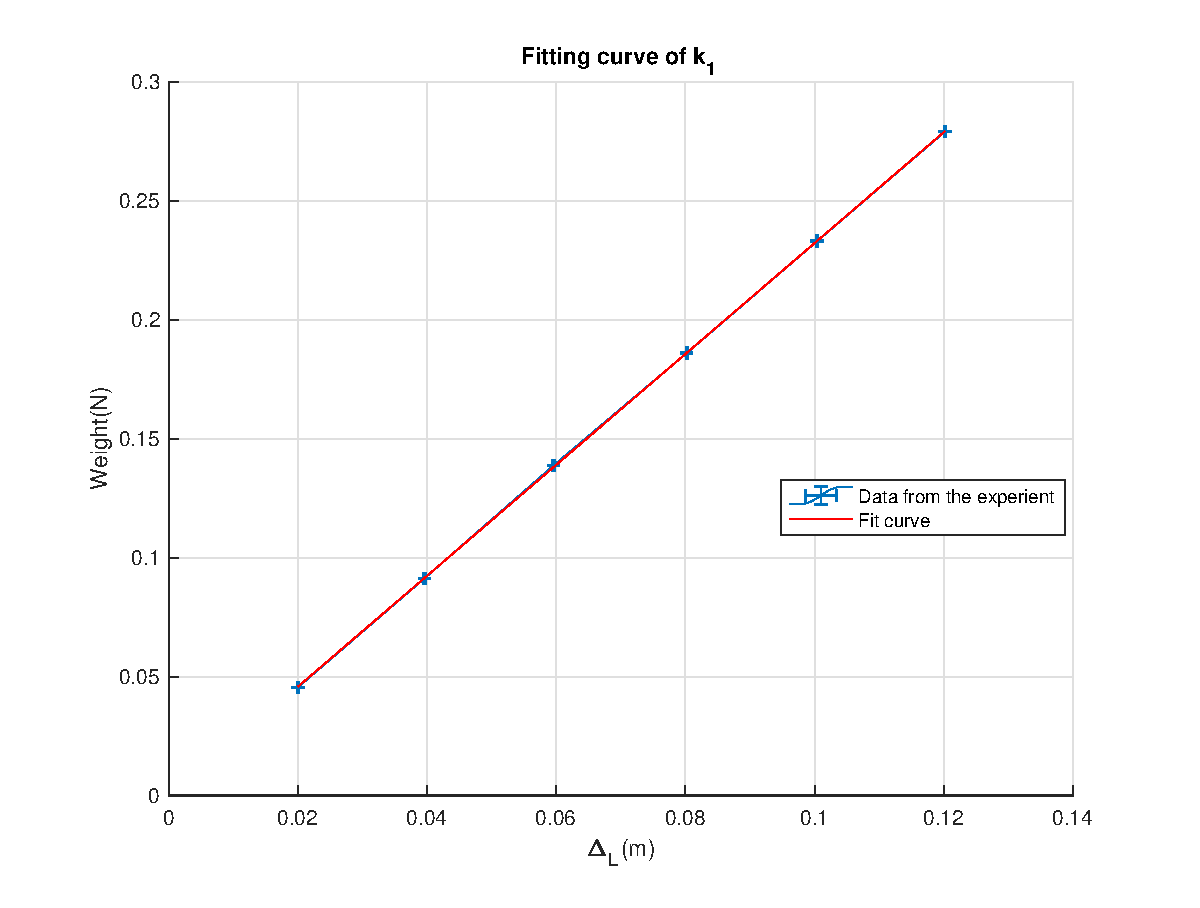
\includegraphics[width=13cm]{matlab/fitfig/k1}
	\caption{Fit curve of spring 1}
\end{figure}

$$ k_1 = 2.3311 \pm 0.013 [N/m] $$
$$ u_{k_1,r} = 0.55 \% $$

Goodness of fit:
\begin{quote}
	\centering
	SSE: 6.091e-07\\
	R-square: 1\\
	Adjusted R-square: 1 \\
	RMSE: 0.0003902 \\
\end{quote}


% =====================================
% NOTE: Spring 2
For Spring 2, we can have its length change data versus the force affected on it
data.  

\begin{table}[H]
	\centering
	\begin{tabular}{|c|c|c|}
	\hline
	No. & length [cm] $\pm$ 0.01 [cm] & F [N] $\pm$ 0.0001 [N] \\ \hline
	$\Delta L_1$ & 2.01  &  0.0455  \\ \hline
	$\Delta L_2$ & 4.00  &  0.0913  \\ \hline
	$\Delta L_3$ & 6.03  &  0.1388  \\ \hline
	$\Delta L_4$ & 8.06  &  0.1860  \\ \hline
	$\Delta L_5$ & 10.08 &  0.2331  \\ \hline
	$\Delta L_6$ & 12.10 &  0.2792  \\ \hline
	\end{tabular}
	\caption{$\Delta L$  vs. Force for Spring 2}
\label{s2df}
\end{table}

Then we use MATLAB fit tools to find $k_2$

\begin{figure}[H]
	\centering
	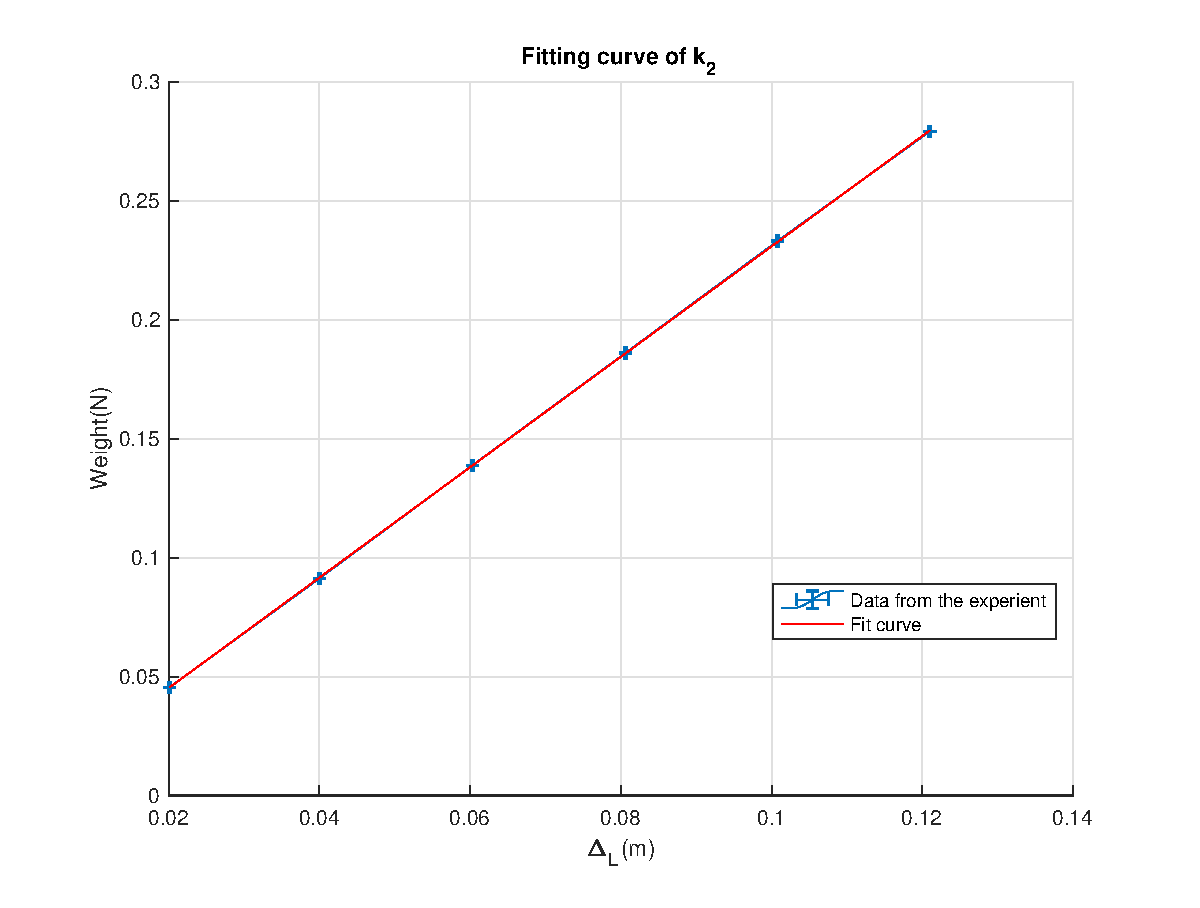
\includegraphics[width=13cm]{matlab/fitfig/k2}
	\caption{Fit curve of spring 2}
\end{figure}

$$k_2 =  2.3206 \pm 0.0105 [N/m] $$
$$ u_{k_2,r} = 0.45 \% $$

Goodness of fit:
\begin{quote}
	\centering
	SSE: 4.305e-07 \\
	R-square: 1 \\
	Adjusted R-square: 1 \\
 	RMSE: 0.0003281 \\
\end{quote}

% =====================================
% NOTE: Spring serial
For serial, we can have its length change data versus the force affected on it
data.  

\begin{table}[H]
	\centering
	\begin{tabular}{|c|c|c|}
	\hline
	No. & length [cm] $\pm$ 0.01 [cm] & F [N] $\pm$ 0.0001 [N] \\ \hline
	$\Delta L_1$ & 3.96  &  0.0455  \\ \hline
	$\Delta L_2$ & 7.94  &  0.0913  \\ \hline
	$\Delta L_3$ & 11.90 &  0.1388  \\ \hline
	$\Delta L_4$ & 16.40 &  0.1860  \\ \hline
	$\Delta L_5$ & 19.94 &  0.2331  \\ \hline
	$\Delta L_6$ & 24.02 &  0.2792  \\ \hline
	\end{tabular}
	\caption{$\Delta L$  vs. Force for serial}
\label{ssdf}
\end{table}

Then we use MATLAB fit tools to find $k_3$ , in other words, the $k$ of the serial string.

\begin{figure}[H]
	\centering
	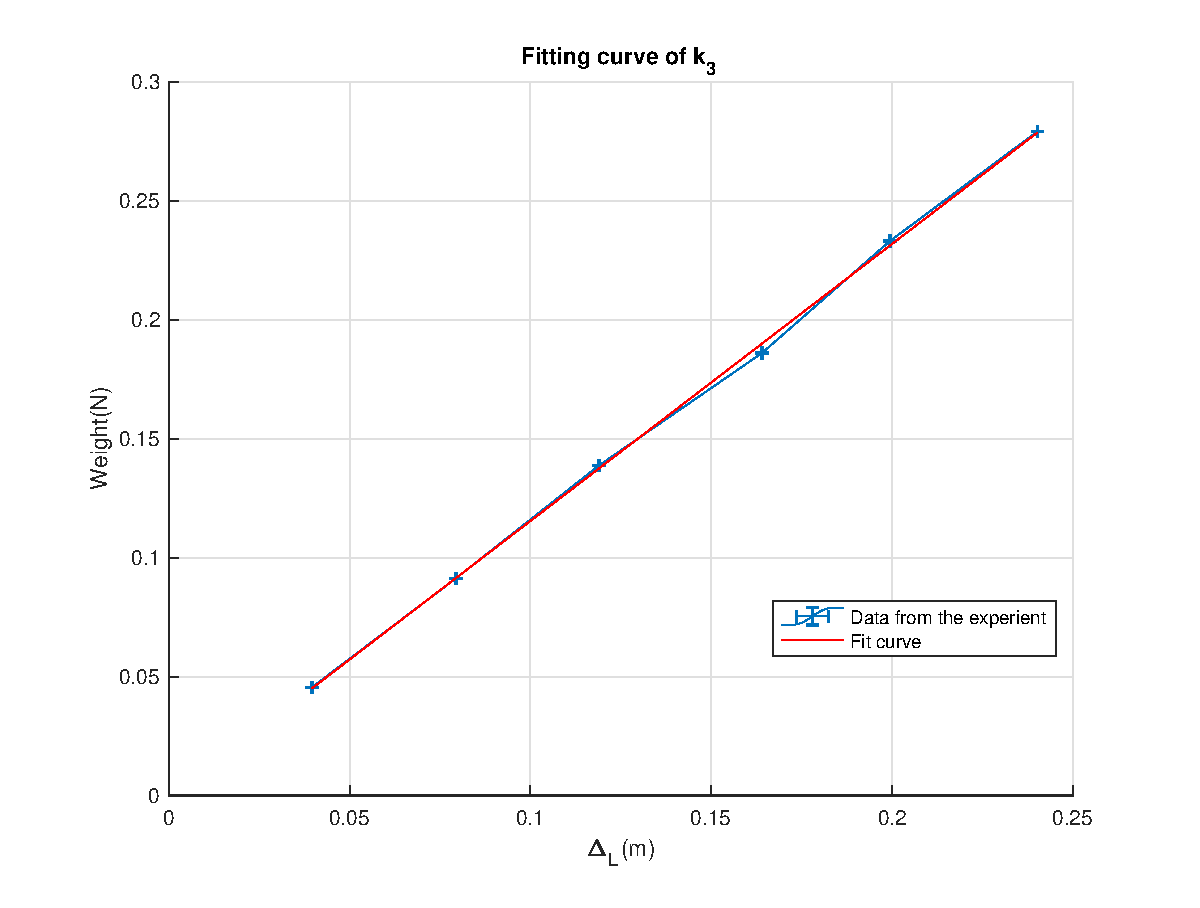
\includegraphics[width=13cm]{matlab/fitfig/k3}
	\caption{Fit curve of spring serial}
\end{figure}

$$k_3 = 1.165 \pm 0.0380 [N/m] $$
$$ u_{k_3,r} = 3.26 \% $$

Goodness of fit:
\begin{quote}
	\centering
	SSE: 2.144e-05 \\
	R-square: 0.9994 \\
	Adjusted R-square: 0.9993 \\
	RMSE: 0.002315  \\
\end{quote}

% NOTE: k cal

By theory, we can calculate $k_3$, i.e. the $k$ of the spring serial by 
$$ k_{3,theory} = \frac{k_1 \cdot k_2 }{k_1 + k_2} =  1.1629 $$ 

Compared with $k_3 = 1.1649$  from the experiment,
$$ u_{k_{3,theory},k_3} = \frac{1.1649 - 1.1629}{1.1629} \cdot 100 \%  = 0.17 \% $$ 
The theory data is close to the experiment data

\subsection{Relation between the period $T$ and the mass $M$}

In this part, we investigate in finding the relation between the period $T$ and 
the mass $M$.
First, we need to collect the mass data needed later for the fit. Shown in Table~\ref{dataMass}.

\begin{table}[H]
	\centering
	\begin{tabular}{|c|c|}
	\hline
	\multicolumn{2}{|c|}{Mass of the object [g] $\pm$ 0.01 [g]} \\ \hline
	object with I-shape $m_{I-obj}$  & 176.87 \\ \hline
	object with U-shape $m_{U-obj}$  & 188.16 \\ \hline
	spring 1 			$m_{spr1}$ & 188.16 \\ \hline
	spring 2 			$m_{spr2}$ & 188.16 \\ \hline \hline
	\multicolumn{2}{|c|}{Mass of the object [g] $\pm$ 0.015 [g]} \\ \hline 
	equivalent mass		$M_{0,I} = m_{I-obj} + \frac{1}{3} m_{spr1} + \frac{1}{3} m_{spr2} $ & 184.13 \\ \hline 
	equivalent mass		$M_{0,U} = m_{U-obj} + \frac{1}{3} m_{spr1} + \frac{1}{3} m_{spr2} $ & 195.42 \\ \hline 
	\end{tabular}
	\caption{Mass measurement data}
\label{dataMass}
\end{table}


The the period $T$ measured in different situations are shown in Table~\ref{dataTime}.

\begin{table}[H]
	\centering
	\begin{tabular}{|c|c||c|c||c|c|}
	\hline
	\multicolumn{6}{|c|}{10 periods [ms] $\pm$ 0.1 [ms]} \\ \hline
    \multicolumn{2}{|c||}{horizontal}  &
     \multicolumn{2}{|c||}{incline 1}  &
     \multicolumn{2}{|c|}{incline 2}  \\ \hline
	$m_1$ & 12560.4 & $m_1$ & 12557.8 & $m_1$ & 12560.9 \\ \hline
	$m_2$ & 12718.2 & $m_2$ & 12711.1 & $m_2$ & 12722.0 \\ \hline
	$m_3$ & 12878.4 & $m_3$ & 12872.2 & $m_3$ & 12885.9 \\ \hline
	$m_4$ & 13021.2 & $m_4$ & 13030.3 & $m_4$ & 13034.7 \\ \hline
	$m_5$ & 13189.2 & $m_5$ & 13186.0 & $m_5$ & 13179.2 \\ \hline
	$m_6$ & 13326.5 & $m_6$ & 13333.3 & $m_6$ & 13336.9 \\ \hline
	\end{tabular}
	\caption{Measurement data for the $T$ vs. $M$ relation}
\label{dataTime}
\end{table}

Recall we have the mass data. 
We need to add the mass of object with I-shape to each $m_i$
Thus, we can have,

\begin{table}[H]
\centering
\begin{tabular}{|c|c|}
\hline
\multicolumn{2}{|c|}{m [g] $\pm$ 0.01 [g]} \\ \hline
1 & 181.52 \\ \hline
2 & 186.19 \\ \hline
3 & 191.04 \\ \hline
4 & 195.86 \\ \hline
5 & 200.67 \\ \hline
6 & 205.38 \\ \hline
\end{tabular}
\caption{Mass measurement data with I-shape and the object.}
\label{massofweight1}
\end{table}

Thus, for horizontal situation, we can get the following table.

\begin{table}[H]
	\centering
	\begin{tabular}{|c|c|}
	\hline
	mass [g] $\pm$ 0.01 [g] & $T^2$ [$s^2$] $\pm$ 0.00001 [$s^2$] \\ \hline
	$m_1$ = 181.52  & 1.57763 \\ \hline
	$m_2$ = 186.19  & 1.61752 \\ \hline
	$m_3$ = 191.04  & 1.65853 \\ \hline
	$m_4$ = 195.86  & 1.69551 \\ \hline
	$m_5$ = 200.67  & 1.73954 \\ \hline
	$m_6$ = 205.38  & 1.77595 \\ \hline
	\end{tabular}
	\caption{$T^2$ vs. $M$ for horizontal situation}
\label{T2vsM_0}
\end{table}

Then we use MATLAB fit tools to find $slope_{h}$

\begin{figure}[H]
	\centering
	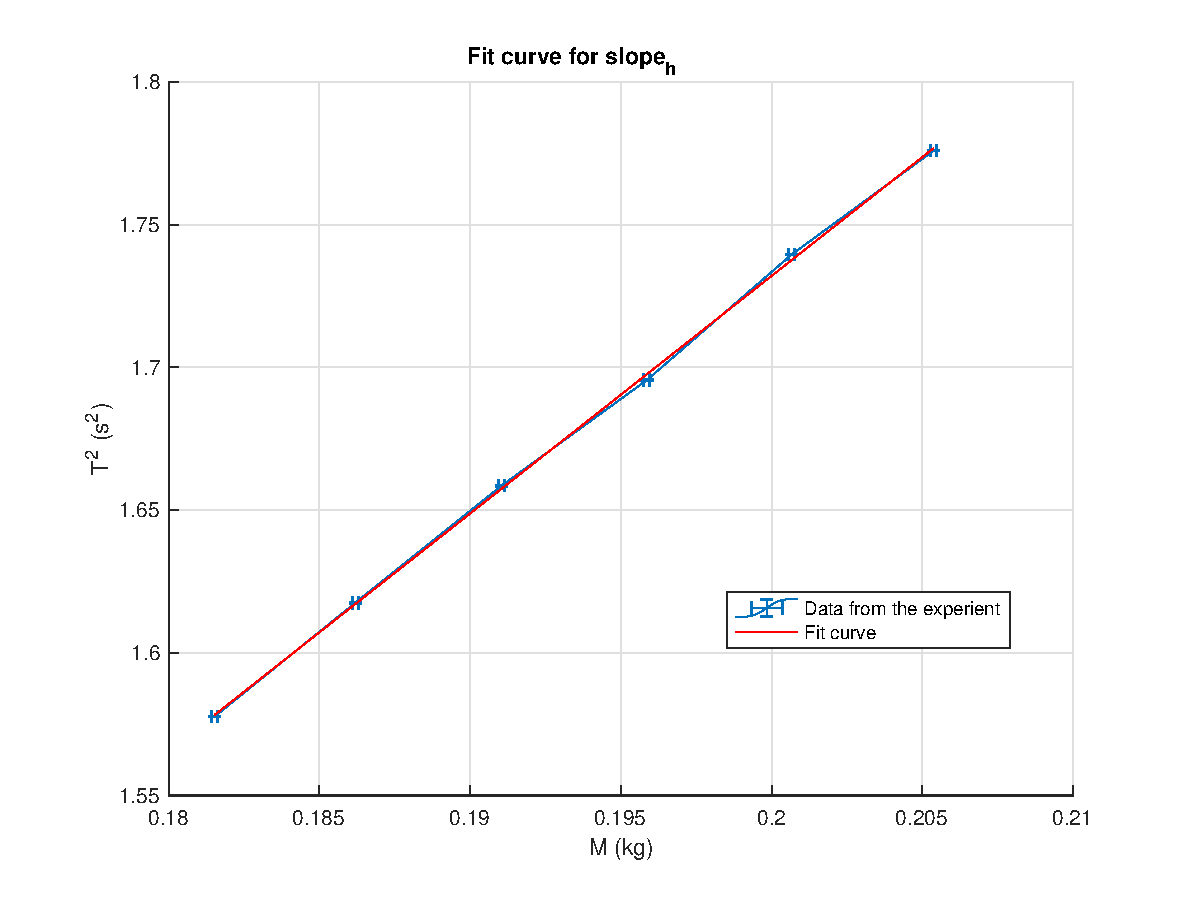
\includegraphics[width=13cm]{matlab/fitfig/m1}
	\caption{Fit curve of $T^2$ vs. $M$ for horizontal situation}
\end{figure}

$$slope_{h} = 8.3233 \pm 0.2235 [s^2/kg] $$
$$ u_{slope_{h},r} = 2.69 \% $$

Goodness of fit:
\begin{quote}
	\centering
  SSE: 1.042e-05 \\ 
  R-square: 0.9996 \\ 
  Adjusted R-square: 0.9995 \\ 
  RMSE: 0.001614 \\
\end{quote}

For incline 1 situation, we can get the following table.

\begin{table}[H]
	\centering
	\begin{tabular}{|c|c|}
	\hline
	mass [g] $\pm$ 0.01 [g] & $T^2$ [$s^2$] $\pm$ 0.00001 [$s^2$] \\ \hline
	$m_1$ = 181.52  & 1.57698 \\ \hline
	$m_2$ = 186.19  & 1.61572 \\ \hline
	$m_3$ = 191.04  & 1.65693 \\ \hline
	$m_4$ = 195.86  & 1.69788 \\ \hline
	$m_5$ = 200.67  & 1.73870 \\ \hline
	$m_6$ = 205.38  & 1.77776 \\ \hline
	\end{tabular}
	\caption{$T^2$ vs. $M$ for incline 1 situation}
\label{T2vsM_1}
\end{table}

Then we use MATLAB fit tools to find $slope_{i1}$, the slope for incline 1.

\begin{figure}[H]
	\centering
	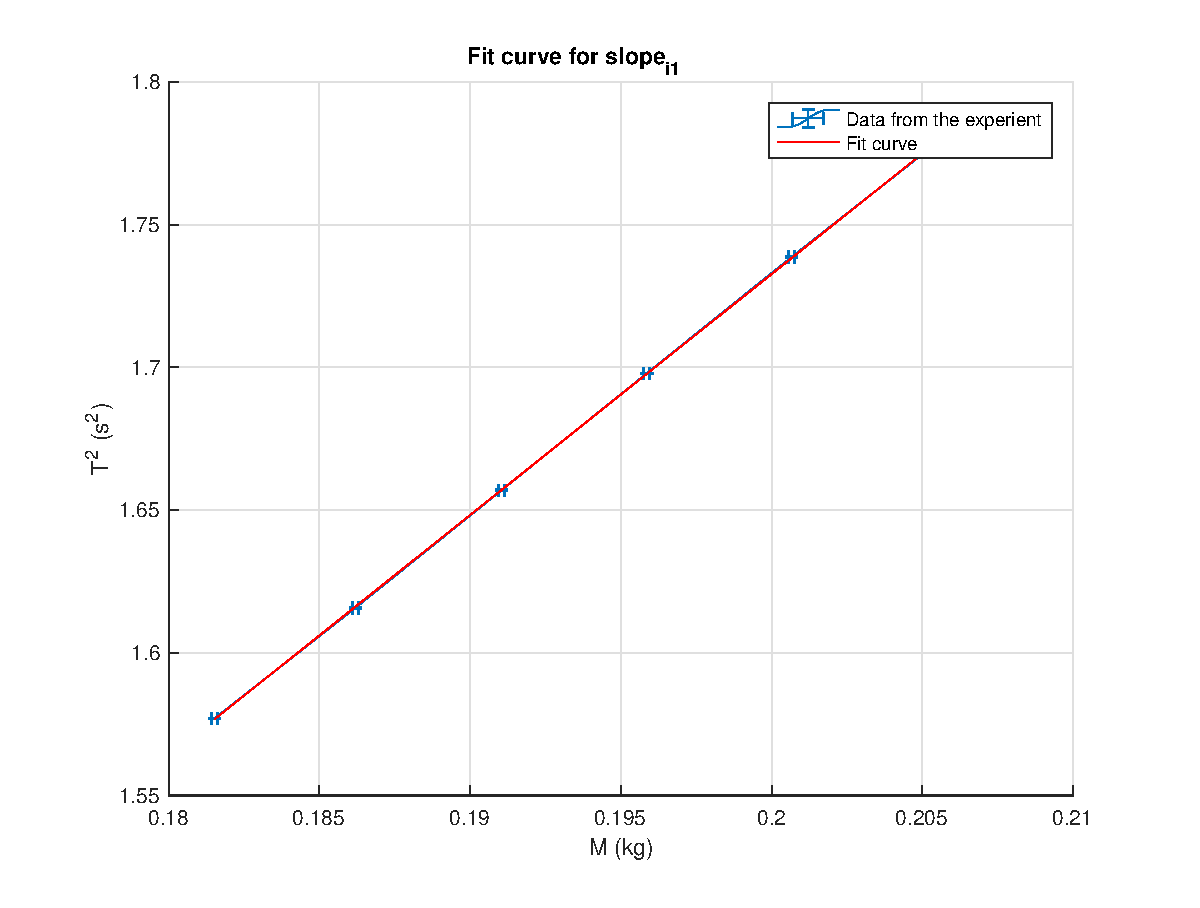
\includegraphics[width=13cm]{matlab/fitfig/m2}
	\caption{Fit curve of $T^2$ vs. $M$ for incline 1 situation}
\end{figure}

$$slope_{i1} = 8.4380 \pm 0.0500 [s^2/kg] $$
$$ u_{slope_{i1},r} = 0.59 \% $$

Goodness of fit:
\begin{quote}
	\centering
  SSE: 5.119e-07 \\ 
  R-square: 1 \\ 
  Adjusted R-square: 1 \\ 
  RMSE: 0.0003577 \\ 
\end{quote}

For incline 2 situation, we can get the following table.

\begin{table}[H]
	\centering
	\begin{tabular}{|c|c|}
	\hline
	mass [g] $\pm$ 0.01 [g] & $T^2$ [$s^2$] $\pm$ 0.00001 [$s^2$] \\ \hline
	$m_1$ = 181.52  & 1.57776 \\ \hline
	$m_2$ = 186.19  & 1.61849 \\ \hline
	$m_3$ = 191.04  & 1.66046 \\ \hline
	$m_4$ = 195.86  & 1.69903 \\ \hline
	$m_5$ = 200.67  & 1.73691 \\ \hline
	$m_6$ = 205.38  & 1.77872 \\ \hline
	\end{tabular}
	\caption{$T^2$ vs. $M$ for incline 2 situation}
\label{T2vsM_2}
\end{table}

Then we use MATLAB fit tools to find $slope_{i2}$, the slope for incline 2.

\begin{figure}[H]
	\centering
	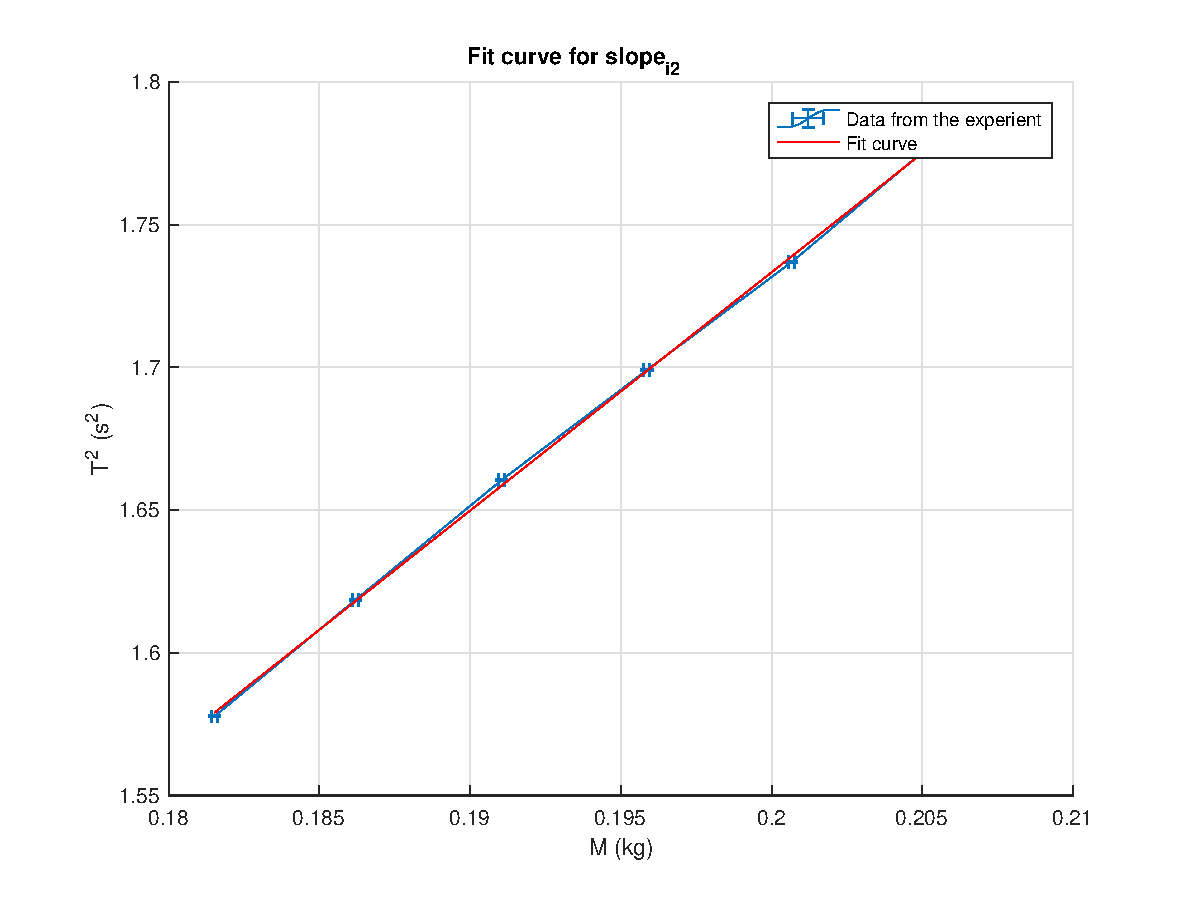
\includegraphics[width=13cm]{matlab/fitfig/m3}
	\caption{Fit curve of $T^2$ vs. $M$ for incline 2 situation}
\end{figure}

$$slope_{i2} = 8.3467 \pm 0.2185 [s^2/kg] $$
$$ u_{slope_{i2},r} = 2.62 \% $$

Goodness of fit:
\begin{quote}
	\centering
  SSE: 9.958e-06 \\
  R-square: 0.9996 \\
  Adjusted R-square: 0.9996 \\
  RMSE: 0.001578 \\
\end{quote}


\subsection{Relation between period $T$ and amplitude $A$}

We get the following raw data from the experiment.
\begin{table}[H]
	\centering
	\begin{tabular}{|c|c|c|}
	\hline
	\multicolumn{2}{|c|}{ $A$ [cm] $\pm$ 0.1 [cm]} & ten periods [ms] $\pm$ 0.1 [ms] \\ \hline
	1 &  5.0 & 12566.3 \\ \hline
	2 & 10.0 & 12565.2 \\ \hline
	3 & 15.0 & 12560.9 \\ \hline
	4 & 20.0 & 12562.6 \\ \hline
	5 & 25.0 & 12562.8 \\ \hline
	6 & 30.0 & 12563.7 \\ \hline
	\end{tabular}
	\caption{ten periods $T$ vs. $A$}
\label{TvsAraw}
\end{table}

Then we can drive it into $T$ vs. $A$

\begin{table}[H]
	\centering
	\begin{tabular}{|c|c|c|}
	\hline
	\multicolumn{2}{|c|}{ $A$ [m] $\pm$ 0.001 [m]} & $T$ [s] $\pm$ 0.00001 [s] \\ \hline
	1 & 0.050 & 1.25663 \\ \hline
	2 & 0.100 & 1.25652 \\ \hline
	3 & 0.150 & 1.25609 \\ \hline
	4 & 0.200 & 1.25626 \\ \hline
	5 & 0.250 & 1.25628 \\ \hline
	6 & 0.300 & 1.25637 \\ \hline
	\end{tabular}
	\caption{$T$ vs. $A$}
\label{TvsA}
\end{table}


\begin{figure}[H]
	\centering
	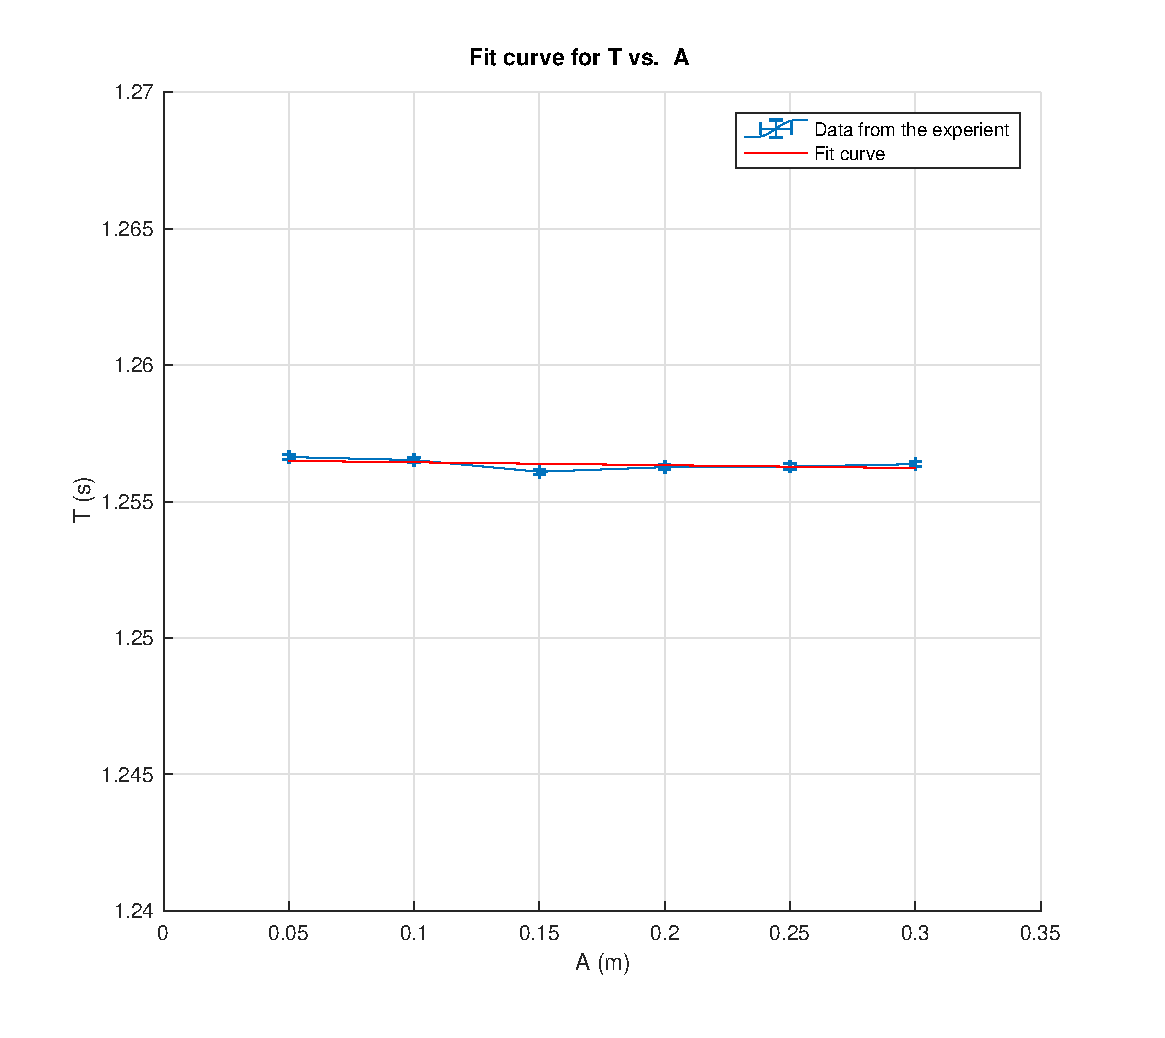
\includegraphics[width=13cm]{matlab/fitfig/a1}
	\caption{Fit curve of $T$ vs. $A$}
\end{figure}

$$ k =  -0.001057 \pm 0.0025  [s/m] $$
$$ u_{k,r} = 236.52 \% $$

Goodness of fit:
\begin{quote}
	\centering
 SSE: 1.39e-07 \\ 
 R-square: 0.2602 \\ 
 Adjusted R-square: 0.07529 \\ 
 RMSE: 0.0001864 \\ 
\end{quote}

For the relative uncertainty is quite large, and R-square is 0.2602, which is not very well,
we can say that $T$ and $A$ do not have a clear linear relation.


\subsection{Relation between $ v_{\max}$ and $A$}

\begin{table}[H]
	\centering
	\begin{tabular}{|c|c|}
	\hline
	$x_{in}$ [cm] $\pm$ 0.002 [cm] & $x_{out}$ [cm] $\pm$ 0.002 [cm]  \\ \hline
	0.472 & 1.542 \\ \hline
	0.482 & 1.540 \\ \hline
	0.480 & 1.530 \\ \hline
	\end{tabular}
	\caption{Data of $x_{in}$ and $x_{out}$}
\label{L_inout}
\end{table}


\begin{table}[H]
	\centering
	\begin{tabular}{|c|c|c|}
	\hline
	\multicolumn{2}{|c|}{ $A$ [cm] $\pm$ 0.1 [cm]} & $\Delta t$ [ms] $\pm$ 0.01 [ms]  \\ \hline
	1  &  5.0 & 42.60 \\ \hline
	2  & 10.0 & 20.56 \\ \hline
	3  & 15.0 & 13.57 \\ \hline
	4  & 20.0 & 10.34 \\ \hline
	5  & 25.0 &  8.25 \\ \hline
	6  & 30.0 &  6.90 \\ \hline
	\end{tabular}
	\caption{Data for the $ {v_{\max}}^2$ vs. $A^2$ relation.}
\label{A_t}
\end{table}


